\documentclass[a4paper,12pt]{article}

\usepackage{fourier}
\usepackage[T1]{fontenc}


\usepackage{lscape}
\usepackage{amsmath}
%\usepackage{framed,enumerate}
%\usepackage{cite}
%\usepackage{color}
\usepackage[usenames,dvipsnames,svgnames,table]{xcolor}
\usepackage[justification=centering]{caption}
\usepackage{ragged2e,float}
\usepackage{subcaption,chngcntr}
%\usepackage[numbered]{mcode}
\usepackage{pgfplots}
\usepackage{tocloft,lipsum}
\usepackage{geometry,graphicx}
\usepackage{tabularx}
\usepackage{multirow}
\usepackage{tabstackengine}
\setstackEOL{@}
\setstackTAB{*}
\geometry{left=20mm,right=20mm,top=20mm,bottom=20mm}
\usepackage{gantt}
\usepackage{tikz}
\usetikzlibrary{shapes,arrows}

% FOR TIKZ AND LABELS
\newlength\figureheight
\newlength\figurewidth
\counterwithin{figure}{section}
\counterwithin{equation}{section}
\counterwithin{table}{section}
%\counterwithin{figure}{subsection}
%\counterwithin{figure}{subsubsect--ion}

% ROBOTO TITLES
\usepackage{titlesec}
\newcommand\roboto[1]{{\usefont{T1}{custom}{m}{n} #1 }}
%\titleformat*{\section}{\Large\roboto}
%\titleformat*{\subsection}{\large\roboto}
%\titleformat*{\subsubsection}{\roboto}
%\renewcommand{\cfttoctitlefont}{\Large\roboto} % contents title
%\renewcommand{\cftloftitlefont}{\Large\roboto} % list of figures title
%\renewcommand{\cftlottitlefont}{\Large\roboto} % list of tables title
\renewcommand{\cftsecleader}{\cftdotfill{\cftdotsep}} % toc dots

% SUBSUBSUBSECTION
\titleclass{\subsubsubsection}{straight}[\subsection]
\newcounter{subsubsubsection}[subsubsection]
\renewcommand\thesubsubsubsection{\thesubsubsection.\arabic{subsubsubsection}}
\titleformat{\subsubsubsection} 
{\normalfont\normalsize\bfseries}{\thesubsubsubsection}{1em}{}
\titlespacing*{\subsubsubsection}
{0pt}{3.25ex plus 1ex minus .2ex}{1.5ex plus .2ex}
\makeatletter
\def\toclevel@subsubsubsection{4}
\def\l@subsubsubsection{\@dottedtocline{4}{7em}{4em}}
\makeatother
\setcounter{secnumdepth}{4}
\setcounter{tocdepth}{4}

\usepackage{fancyhdr}
\pagestyle{fancy}
\fancyhf{}
\renewcommand{\headrulewidth}{0pt}
\rfoot{\thepage}
\lfoot{\textcolor{gray}{CubeSat Design Overview Report}} 

\usepackage{setspace}
%\singlespacing
%\onehalfspacing
%\doublespacing
\setstretch{1.1}

%TABLES
\usepackage{array}
\newcolumntype{L}[1]{>{\raggedright\let\newline\\\arraybackslash\hspace{0pt}}m{#1}}
\newcolumntype{C}[1]{>{\centering\let\newline\\\arraybackslash\hspace{0pt}}m{#1}}
\newcolumntype{R}[1]{>{\raggedleft\let\newline\\\arraybackslash\hspace{0pt}}m{#1}}


% SHORTCUTS
\renewcommand{\deg}{\ensuremath{^\circ}}
%\newcommand{\F}[1]{\ensuremath{F_{#1}}}
%\newcommand{\M}[1]{\ensuremath{M_{#1}}}
\newcommand{\tf}[2]{G_{\delta_#1}^{#2}(s)}
\newcommand{\bmat}[2]{\setstackgap{L}{1.2\baselineskip} \fixTABwidth{T} \setstacktabbedgap{#1} \bracketMatrixstack{#2}}
\newcommand{\vertmat}[2]{\setstackgap{L}{1.2\baselineskip} \fixTABwidth{T} \setstacktabbedgap{#1} \vertMatrixstack{#2}}
\newcommand{\tikzpic}[4]{\centering 
    \setlength\figurewidth{#1\linewidth} \setlength\figureheight{#2\linewidth} \input{#3} \caption{#4}}
\newcommand{\pic}[3]{\centering 
    \includegraphics[width=#1\linewidth]{#2} \caption{#3}}
%\newcommand{\unit}[2]{\frac{\text{#1}}{\text{#2}}}

\begin{document}
    
\begin{titlepage}

\thispagestyle{empty}
\begin{center}
\begin{minipage}{\linewidth}
    \centering
%University logo
    
\includegraphics[width=6.5cm]{logo.png}
    \par
    \vspace{1.2cm}
    {\textsc{School of Aerospace Mechanical and Mechatronic Engineering \\ \vspace{0.3cm}
            AERO3760: Space Engineering 2}}
   \vspace{0.7cm}
%Thesis title
	\hrule
    \vspace{1cm}
    {{\LARGE\bf{ Group E: SnapSat\\\vspace{0.4cm}Data Package Document 1 \\Critical Design Review }\par}}

    \vspace{1cm}
    \hrule
    \vspace{1.3cm}
     {\large \textsc{21 August 2015}}
\vspace{1.3cm}
%Author's name
    \begin{table}[H]
        \centering
        %\caption{Team Member Details and Contributions}
        \vspace{0.2cm}
        \label{tab:maxturbulencealpha}
        {\renewcommand{\arraystretch}{1.7}%
            \begin{tabular}{|>{\centering\arraybackslash}m{6cm}|>{\centering\arraybackslash}m{9cm}|}
                \hline
                \textbf{Name and Email} & \textbf{Role and Responsibility} \\ \hline\hline
                James Allworth | 312073038  jall8741@uni.sydney.edu.au & \textit{Attitude Determination and Control System} \newline TASKS  \\\hline
                Thomas Forbutt | 312101058  tfor8012@uni.sydney.edu.au & \textit{Communications and Data Handling} \newline TASKS \\\hline
                Oscar McNulty | 312106130  omcn3220@uni.sydney.edu.au & \textit{Structural Design and Development} \newline TASKS \\\hline
                Penelope Player | 312106718  ppla7388@uni.sydney.edu.au & \textit{On-board Computer and Power System} \newline TASKS \\\hline
                Nikita Sardesai | 312088205  nsar2497@uni.sydney.edu.au & \textit{Thermal System Design and Payload} \newline TASKS \\\hline
                \end{tabular} } 
        \end{table}
    
%    \vspace{1.8cm}
%    {\large\roboto{ Abstract}}
%    \vspace{0.4cm}
%    \justify
%    {\begin{spacing}{1.3} \lipsum[10] \end{spacing}\par}
\end{minipage}
\end{center}

\end{titlepage}


 \begin{table}[H]
     \centering
     \caption{caption}
     \vspace{0.2cm}
     \label{tab:}
     {\renewcommand{\arraystretch}{1.7}%
         \begin{tabular}{|>{\centering\arraybackslash}m{6cm}|>{\centering\arraybackslash}m{9cm}|}
             
             \end{tabular} } 
        \end{table}


\newpage
\tableofcontents
\listoffigures
\listoftables

\newpage
\section{System Overview}
\textit{SnapSat} is an undergraduate project taken on by five students at the University of Sydney. The report will detail the Critical Design Review and specifications that were built to over the 12 week semester. The details of the subsystems and the system integration will be detailed here. The initial design point was for a three month mission at an orbit altitude of 350 kilometres and an inclination of 98\deg. However, this report will mainly detail the requirements for a 30km high-altitude balloon launch. Recommendations and upgrades to make this project viable for the initial design point will be made appropriately.


\subsection{Mission and Objectives}
The main mission of \textit{SnapSat} is to provide a platform to make space activities more accessible to the general public. The aim is to exploit popular social media and to allow the end user to post Twitter updates (Tweets) along with photographs of the Earth from the satellite. In order to do this, the cubesat needs a camera with sufficient resolution to see general country regions (and possible cities) along with a reliable communications connection to allow for fast data transfer at an orbit altitude of 350 kilometres. 
 
\subsection{Components and Subsystems}
On a primary level, for the deign on a high-altitude balloon, the main payload is the camera. Other basic requirements for the launch (power and communications) will be outlined in the following sections and discussed in detail later on in the report. An Attitude Determination and Control Subsystem (ADCS) was also tested and implemented as a proof-of-concept. The full structure was designed in-house and was a conventional laser-cut aluminium chassis. Details of the subsystems and the components chosen to meet each task are detailed in table~\ref{tab:components} below. The budget for the project was \$1000 provided by the School of Aerospace, Mechanical and Mechatronic Engineering at the University of Sydney. Components were selected based on their suitability for the project and for their cost. It was also important to take into consideration the working of other teams within the course. The communications structure chose relies on a `mother' satellite, through which all communications are managed. Components were selected to allow for this to work effectively. The purpose of having a mother sate little was to allow for an easy find after the high altitude balloon launch. 

\begin{table}[H]
   \centering
   \caption{Overview of componenet selection}
   \vspace{0.2cm}
   \label{tab:components}
   {\renewcommand{\arraystretch}{1.4}%
   \begin{tabular}{|>{\arraybackslash}m{3cm}|>{\arraybackslash}m{12cm}|}
         \hline
         \textbf{Subsystem} & \textbf{Chosen Components} \\\hline\hline
         Structural & 	 - industrial grade Aluminium\newline
                         - laser cut, bent to shape and riveted together with M3 threaded rods to supports the Printed Circuit Boards (PCBs)\\\hline
         ADCS & 		 - air-core magnetorquers designed and made in house\newline
                         - OSRAM SFH203P photodiodes to track Sun location\newline
                         - Inertial Measurement Unit (IMU) to obtain gyroscopic data: Adafruit 10-DOF\\\hline
         EPS & - 9cm $\times$ 9cm solar 			panels\newline
                         - 2 $\times$ LiNiMnCo 26650 rechargeable cells\newline
                         - Adafruit voltage regulators\\\hline
         OBC/OBDH & - Microcontroller: Iduino DUE (Arduino DUE clone)\newline
                         - PCB $\times$ 4: power board, control systems and payload board, communications board, microcontroller board\\\hline
         TT\&C &
                         - RF 900 chip\newline
                         - duck antennae\newline
                         - Ublox 3.3V GPS\\\hline
         Thermal & 		 - passive coatings on cubesat chassis: kapton tape\\\hline
         Payload & 		 - camera: Arducam mini\\\hline  
   \end{tabular} } 
\end{table}

\subsection{System Integration}
Figure~\ref{fig:integration} below shows the schematic of how all the subsystems will work together and their communication protocol.
\begin{figure}[H]
    \centering
    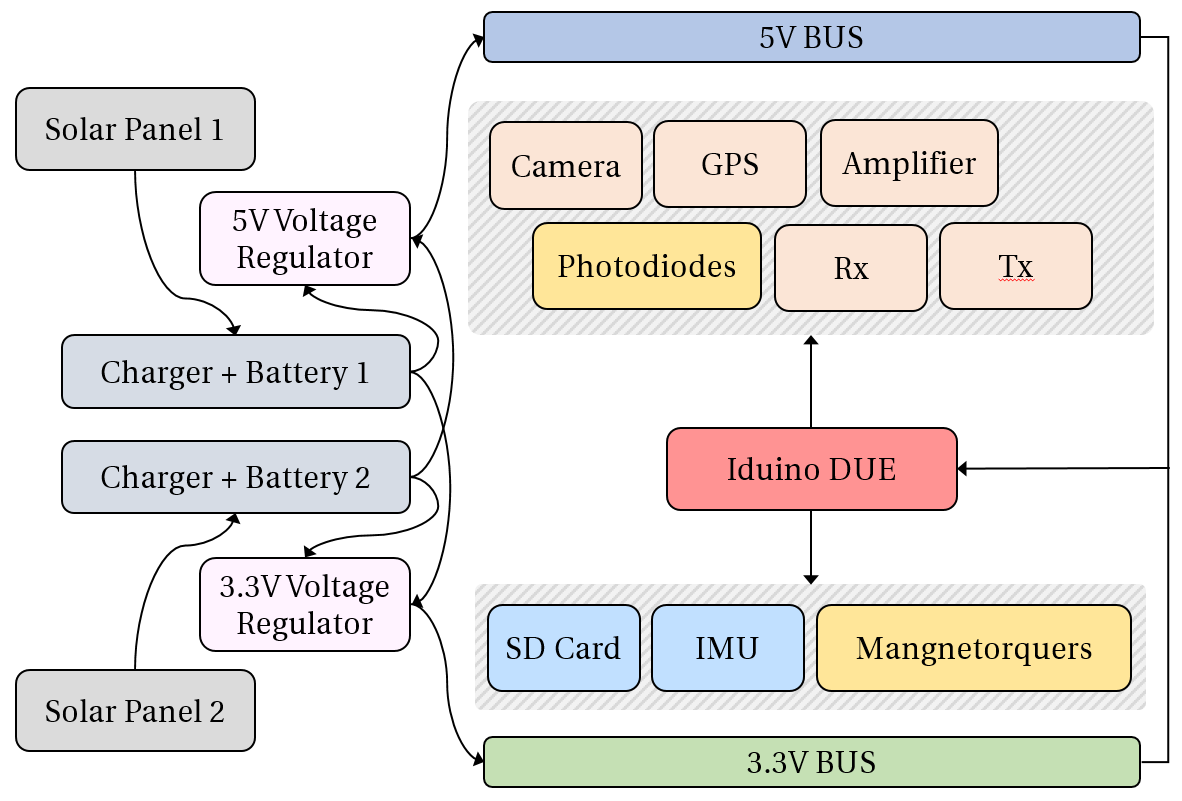
\includegraphics[width=0.75\linewidth]{./figures/integration}
    \caption{Full System Integration}
    \label{fig:integration}
\end{figure}


\newpage
\section{Payload Design}

\newpage
\section{Structural Subsystem}

\newpage
\section{Attitude Determination and Control Subsystem}
\subsection{Inertial Measurement Unit}
The inertial measurement unit (IMU) that was selected for the balloon launch is a 10 degree of freedom (DOF) Adafruit IMU.  It includes a 3DOF magnetometer, a 3D0F accelerometer and a 3DOF gyroscope as well as a barometric pressure/altitude sensor which also includes temperature.  The IMU uses an Attidude Heading and Reference System (AHRS) algorithm that returns the pitch, yaw and roll of the satellite with respect to magnetic north.  Given the fact that this is a very cheap IMU there is a degree of drift associated with the gyroscope which causes inaccuracies.  There is also an error associated with the accelerometer however it is less than the the drift caused by the gyroscope. As such the accelerometer has been used to determine the attitude both for the balloon launch and in the functional testing as the photodiode system will not be functional in either of these tests.\\


In terms of the application in space for this component, the major problem with this IMU is that it is not radiation hardened which will result in larger errors the longer it remains in orbit and will eventually cause it to stop working.  Thus in the event of an actual space launch, this component would need to be replaced with a radiation and preferably more accurate component.  The other major error that effects the IMU is accumulated error which is directly related to the amount of time spent in orbit.  Although this may be reduced in higher quality IMU's it will always be an issue.  Thus a secondary orientation system is required in order to determine the attitude of the SnapSat accurately.

\subsection{Photodiode Sun Sensor System}
A photodiode based sun sensor system was selected to be the secondary orientation system in order to recalibrate the IMU and to use in long duration missions.  This system was primarily selected because it provides enough pointing accuracy for the purposes of this mission and is significantly cheaper than the alternatives of star trackers or actual sun sensors.  The actual component that was selected is an OSRAM SFH203P Photodiode.  Although these are simply off the shelf components, a cover glass can be placed over the photodiodes in order to protect them from UV radiation.



\section{Selection of Magnetorquers}
The SnapSat is a relatively small satellite with low mass and power considerations.
After extensive literature review it was determined that given the mass and power consideration of the SnapSat, magnetorquers would provide a better controls system than 

\section{Design of Magnetorquer}
The torque on the satellite produced by the magnetorquer is given by cross product of the magnetic dipole of the magnetorquer and the earths magnetic field strength: 
\begin{center}
$T = M \times B$
\end{center}
It is impossible to change the earth's magnetic field strength which is approximately $3 \times 10^{-6}$ Tesla.  Thus in order to maximise the torque on the satellite the magnetic dipole must be maximised. The magnetic dipole for the magnetorquer is given by the following equation:
\begin{center}
$M = N \cdot I \cdot A$
\end{center}
Thus the magnetic dipole is dependent on the number of turns in the coil, the current through the wire and the area of the coil.  Initially it seems like a simple problem where the dipole will simply increase with the number of turns if the current and area are held constant.  However, this view does not take into account the resistance that increases with the length of wire, which given the fixed voltage will limit the current.  Due to cost restrictions, only 0.18mm round copper wire was available for use, which had a resistance per metre ($R_m$) of 0.646 ohms.  The following equations were then combined with the magnetic dipole equation in order to optimise the number of turns required:
\begin{center}
$I = \frac{V}{R}$\vspace{2mm}\\
$R = N \cdot Perimeter \cdot R_m$ \vspace{2mm}\\
$P = V \cdot I$
\end{center}
When combined the following equation was determined:
\begin{center}
$1 = \frac{4 \cdot M \cdot R_m}{V \cdot A}$
\end{center}
Thus since resistance per metre and voltage are constant, and perimeter is dependent on area, the magnetic dipole becomes constant for a given area.  Due to the restrictions in the lab only two sizes were available for the magnetorquers. The larger size was selected with side lengths of 0.073m as when the smaller size was modelled, the current draw was too high causing a higher level of power to be used.  Thus given this fixed area, the maximum magnetic dipole was determined to be  0.14$Am^2$.  Using this maximum dipole as the basis, the other characteristics of the magnetorquer were determined and can be viewed in the table below.




\begin{table}[H]
\begin{center}
\caption{Predicted Data for the Magnetorquers}
\begin{tabular}{|c|c|c|c|c|c|c|c|}
\hline
Magnetic Dipole & Number of Turns & Current & Area & Voltage & Resistance & Power Required\\
\hline
0.14$Am^2$ & 132 & 0.2A & 0.005329$m^2$ & 5V & 24.9$\Omega$ & 1W\\
\hline
\end{tabular}
\end{center}
\vspace{-6mm}
\end{table}

\section{Construction of Magnetorquers}
As mentioned previously the Magnetorquers were built in house using equipment provided in the space lab.  The following procedure was applied to make each magnetorquer:
\begin{enumerate}
	\item The metal structural mould for the magnetorquer was unscrewed and sticky tape was applied to areas that were likely to come into contact with glue.
	\item The mould was placed in the winder and the copper wire was set up as shown in the photographs below.
	\begin{center}
	\begin{figure}[H]
	\caption{Magnetorquer Construction Set Up}
	\begin{subfigure}{0.5\textwidth}
	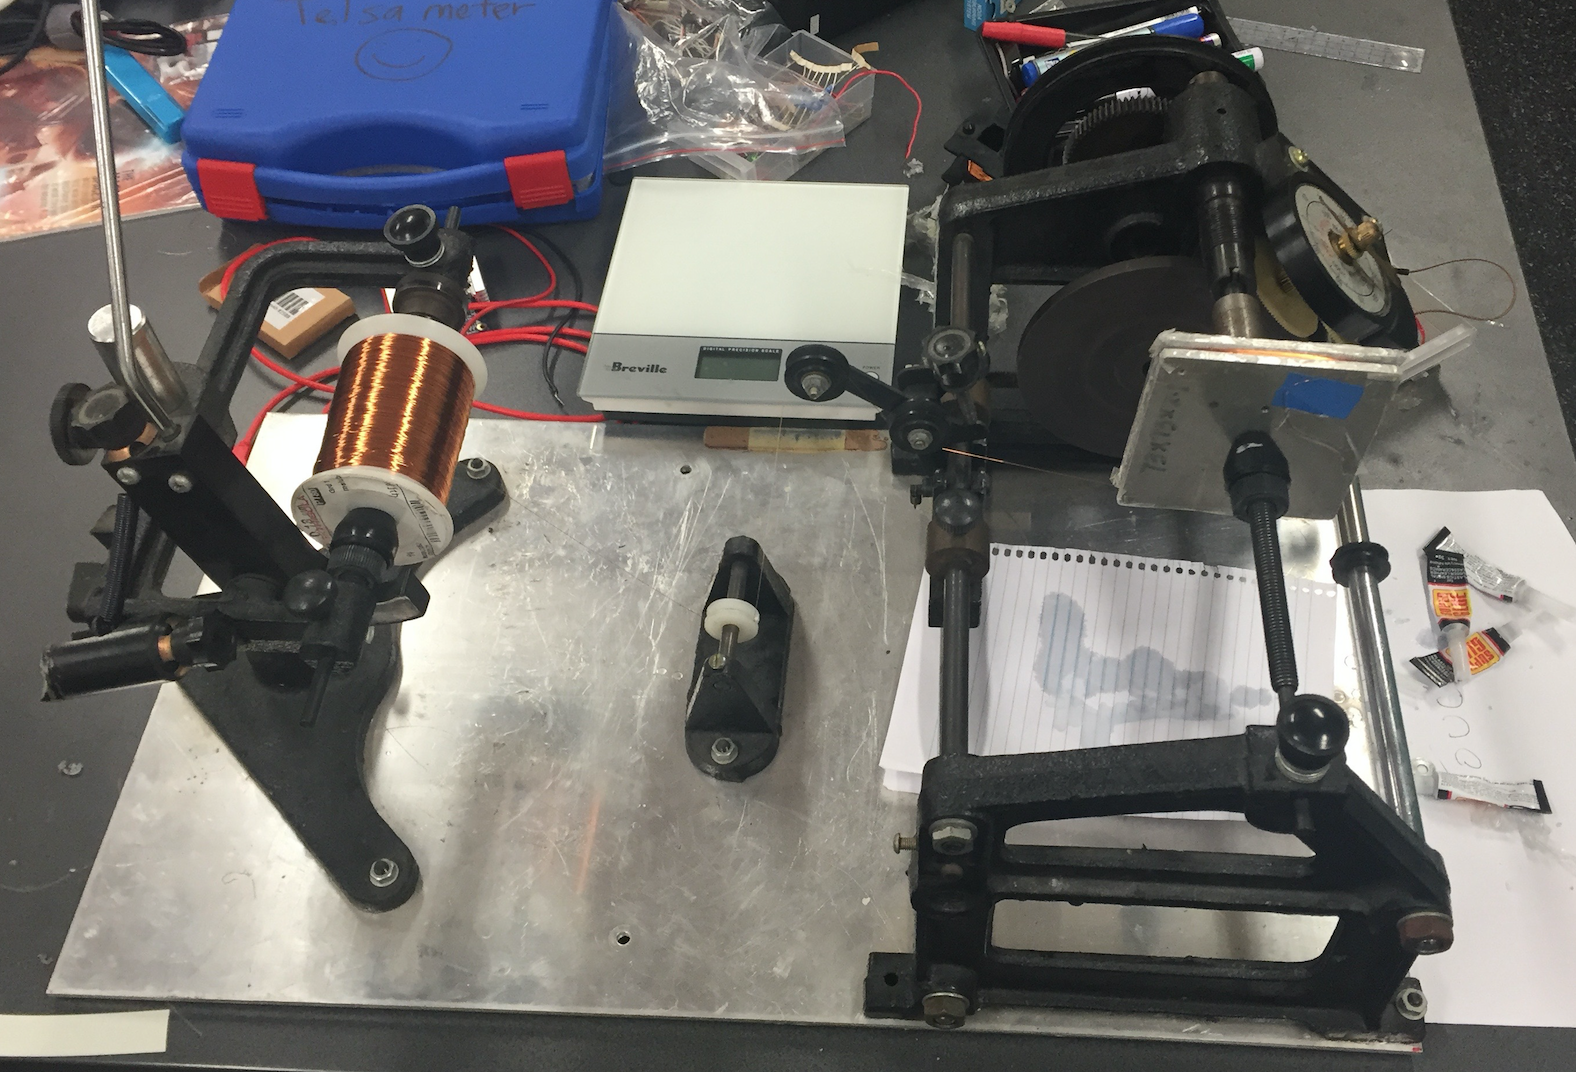
\includegraphics[scale = 0.35]{Construction_1.png}
	\end{subfigure}
	\hspace{10mm}
	\begin{subfigure}{0.5\textwidth}
	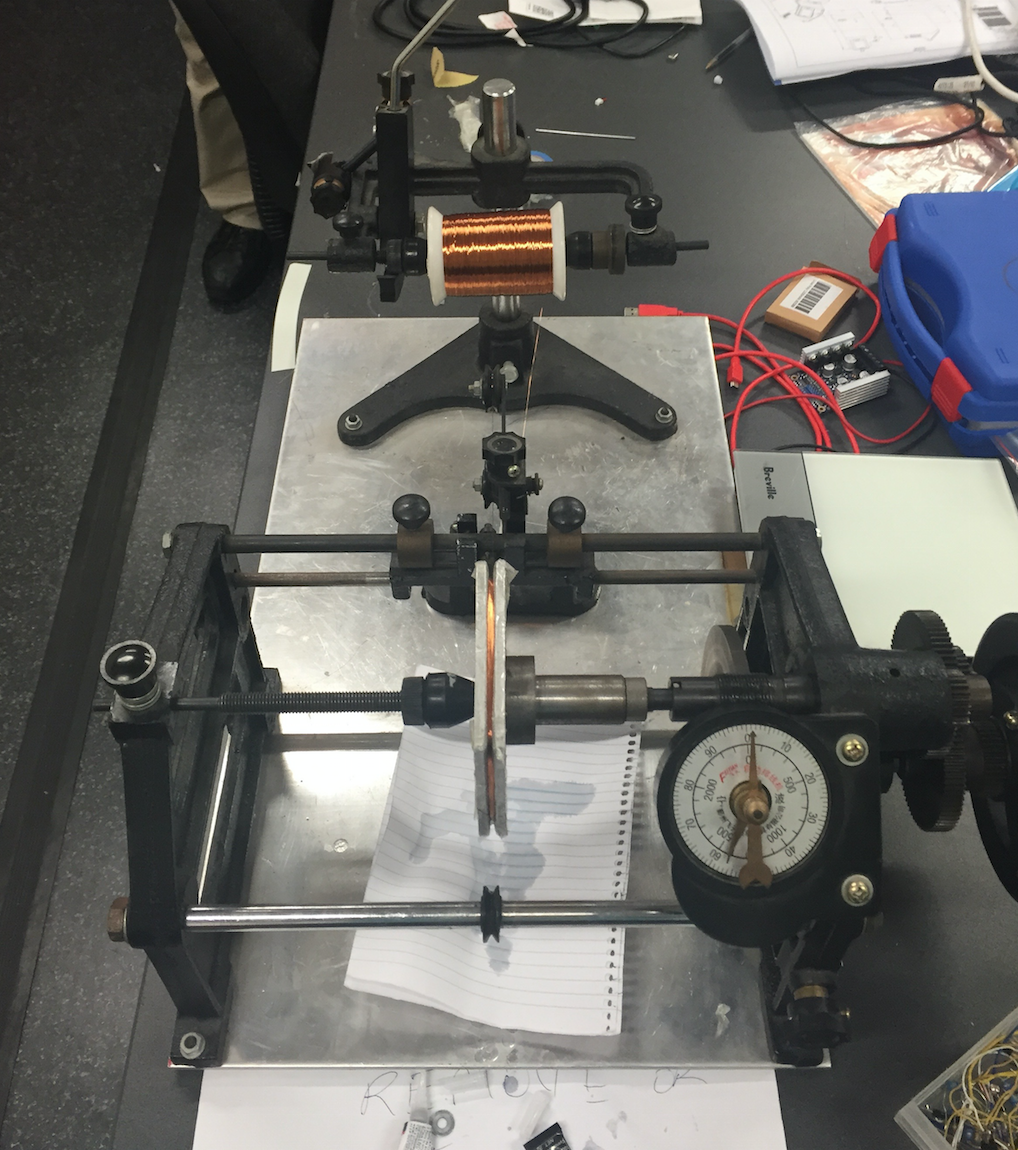
\includegraphics[scale = 0.35]{Construction_2.png}
	\end{subfigure}
	\end{figure}
	\end{center}
	\vspace{-5mm}
	
	
	\item The wire at the very beginning of the coil was taped to the side of the mould to keep it separate from the coil so that it can be connected to the PCB.
	\item In order to measure the number of turns, the counter on the winder was set to zero.
	\item Twenty turns were completed and then a layer of super glue was added to the coiled wire on all four sides in order using a thin brush.
	\item Step 4 was repeated until the required number of turns was reached at which point another layer of glue was added to each side of the coil.
	\item The copper wire was cut and the wire at the very end of the coil was not stuck to the the main coil in order to provide a connection between the PCB and the magnetorquer.
	\item The glue was allowed to set for 10 mins and then the coil was carefully removed from the mould with the aid of the sticky tape.
	\item Once completed the ends of coil were carefully scraped with sandpaper in order to remove the protective coating and allow current to be passed through.
	\item The coil was testing by attaching it to a battery and using a compass to determine whether a magnetic field was being produced.
	\item An Ohmmeter was used to determine the resistance through the coil.  
\end{enumerate}
After testing both magnetorquers were found to have a slightly higher resistance than predicted with the first magnetorquer reading a resistance of 27.2$\Omega$ and the second magnetorquer reading 28.1$\Omega$.  This is roughly a 10\% increase on the predicted value of 24.9$\Omega$ and is most likely caused by the effect of the super glue which was not taken into consideration in the original calculations.  This will result in the magnetorquers using a slightly lower current as voltage is constant and have a lower maximum dipole value.  These values were calculated to be 0.138$Am^2$ and 0.137$Am^2$ for magnetorquers 1 and 2 respectively.  The image below depicts magnetorquer 1 just after construction.

\vspace{-6mm}
\begin{center}
\begin{figure}[H]
\caption{Completed Magnetorquer}
\vspace{-4mm}
\centering
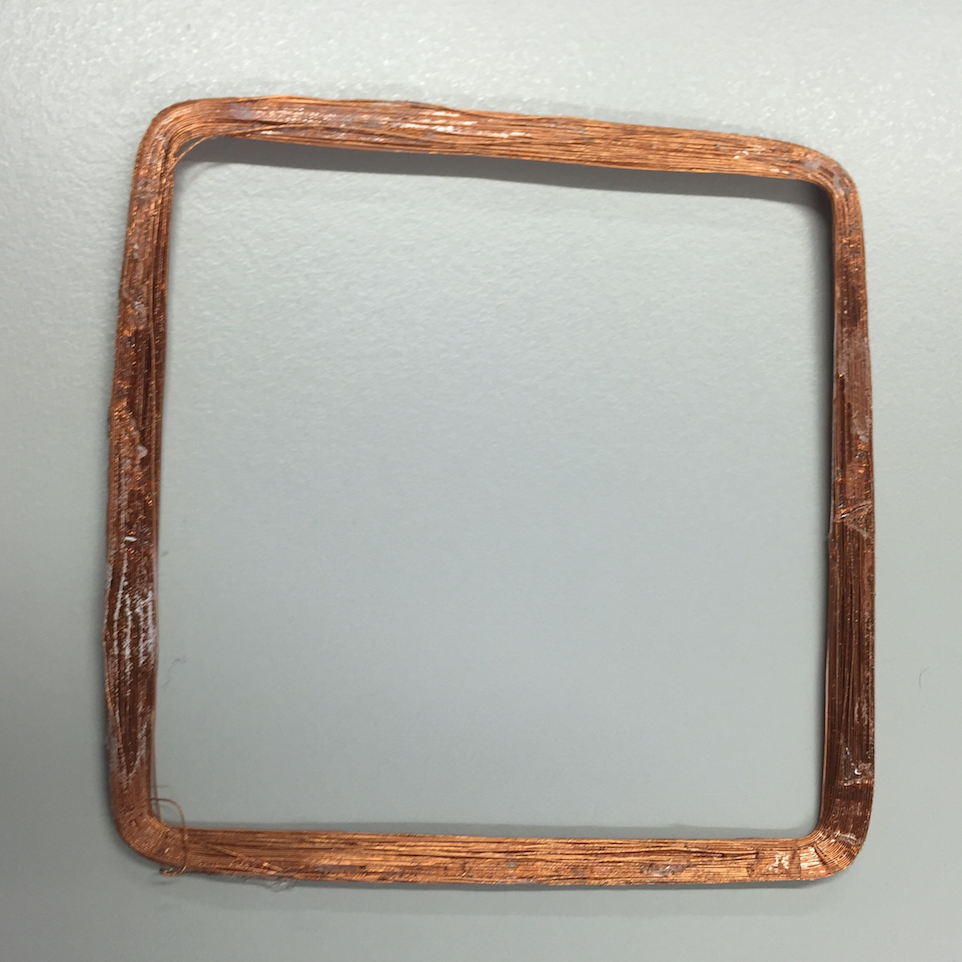
\includegraphics[scale = 0.4]{Magnetorquer.png}
\end{figure}
\end{center}
\vspace{-5mm}

\section{Magnetorquer Control System}
The dynamic model for the magnetorquer control system was produced by three fundamental equations:
\begin{center}
$T = N \cdot I \cdot A \cdot B \cdot sin(\theta)$ \vspace{2mm} \\
$V = I \cdot R$\vspace{2mm}\\
$T = J \cdot \ddot{\theta}$\\
\end{center}
By combining these three equations and using a Laplace transform the following dynamic model was determined:
\begin{center}
$\frac{\theta(s)}{V(s)} = \frac{N \cdot A \cdot B}{J \cdot R \cdot s^2 (s^2 + 1)}$
\end{center}
Thus using this function the following Simulink model was produced to determine the expected response of the satellite given certain inputs.

\vspace{-6mm}
\begin{center}`
\begin{figure}[H]
\caption{Simulink Model of Control System}
\vspace{-4mm}
\centering
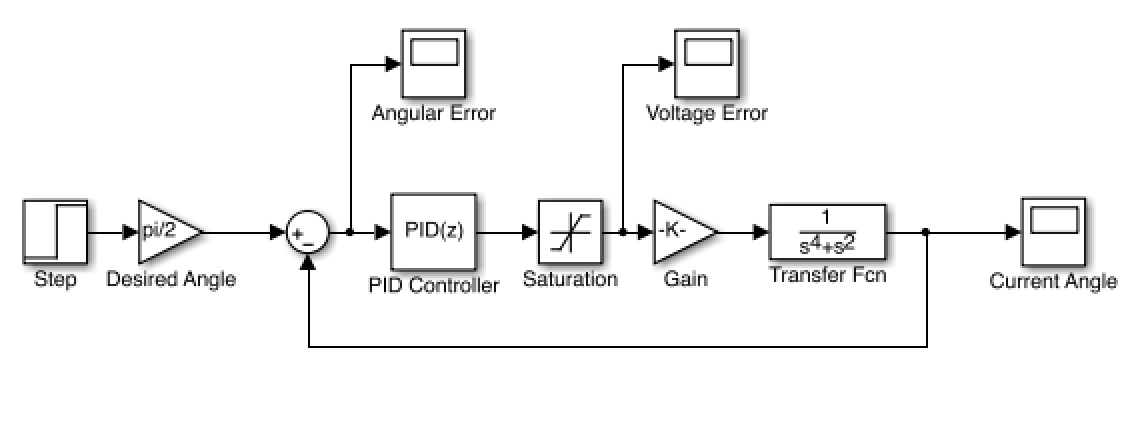
\includegraphics[scale = 0.8]{Simulink_ADCS_Model.png}
\end{figure}
\end{center}
\vspace{-5mm}


\newpage
\section{Electrical Power Subsystem}

\newpage
\section{On-Board Computer and On-board Data Handling Subsystem}

The SnapSat uses an Iduino Due Pro MCU to control the operation of the modules.  It does not use an RTOS, instead using an infinite loop to log image and location data, but interrupt based control to priorities incoming messages of the communications subsystem. \\

FBD OF PROGRAM STRUCTURE \\

All data is logged on the SD Card 

\newpage
\section{Communications Subsystem}
The communications system that was decided upon consists of a RFD 900+ transceiver that is linked to a ground station and other satellites with the same chip. The transceiver chip is connected to two antennas that increase gain allowing for larger uplink and downlink margins. The chip communicates to the OBC via UART and for a simple two node communication system works out of the box. For recovery purposes it was decided the satellites to be launched at the same time as SnapSat will be linked together via a multipoint network. 

\noindent
The requirements of the communication system include emitting a beacon containing the whole orbit data (WOD) collected every 30 seconds. IT must also be able to accept commands from the ground station and send back payload data to earth. An example of the commands this system is able to receive and execute are turning transmissions on and off to control which satellite is emitting at a set time.

\subsection{Componenets}
\begin{figure}[H]
    \centering
    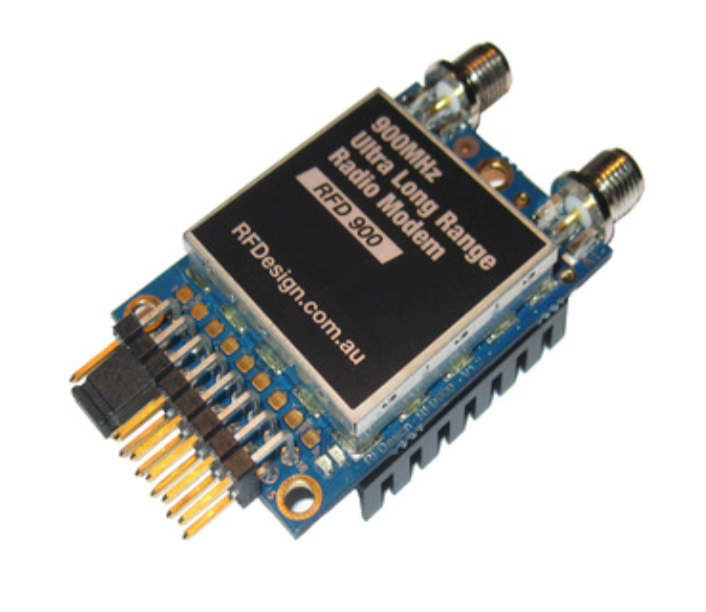
\includegraphics[width=0.6\linewidth]{./figures/rfd}
    \caption{RFD900}
\end{figure}
\noindent
As mentioned above the core of the communications subsystem is the RFD 900+ transceiver from RFDesigns. It was decided that the Arduino shield used to interface the transceiver with the OBC was not necessary and direct soldering on to our PCBs would allow for a more compact design. To complete this the following pins were connected to the associated Arduino pins with data in from the transceiver connecting to data out of the Arduino and vice versa. 
\begin{figure}[H]
\centering
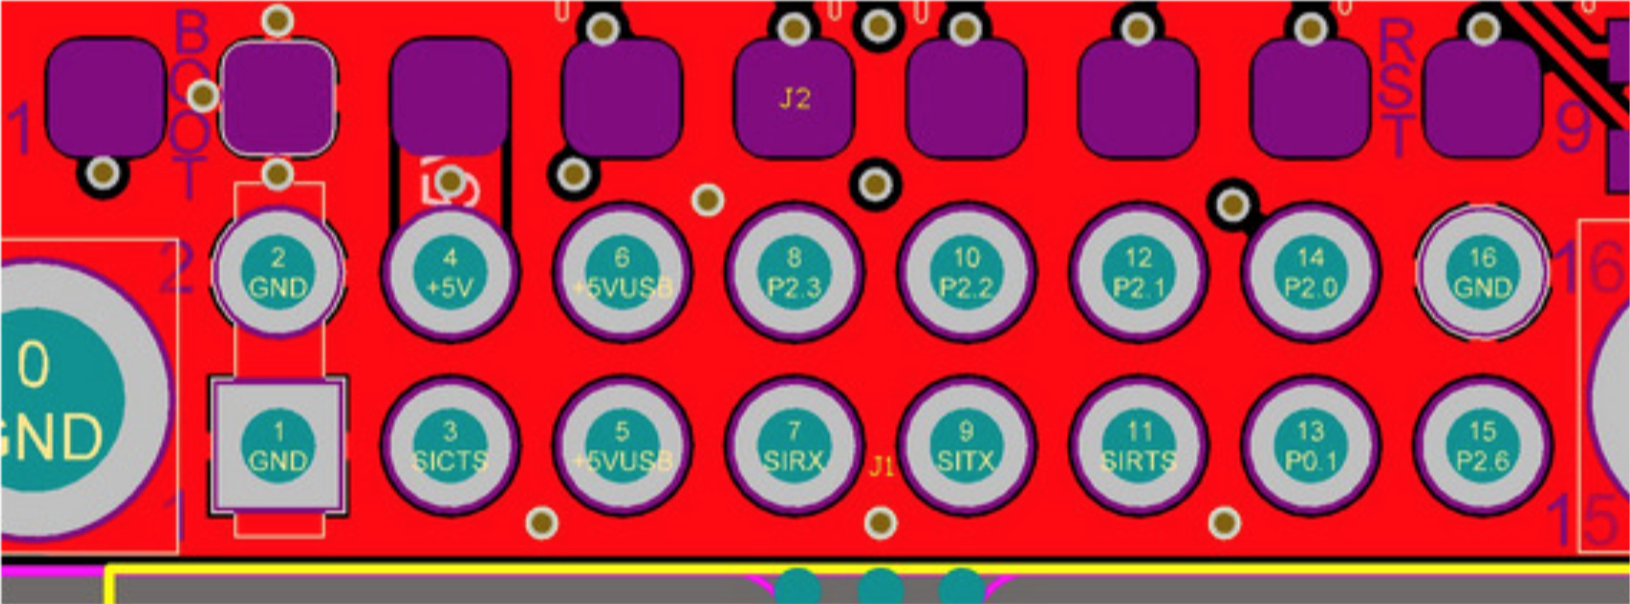
\includegraphics[width=\linewidth]{./figures/pins}
\caption{Pin Diagram}
\end{figure}
\begin{figure}[H]
    \centering
    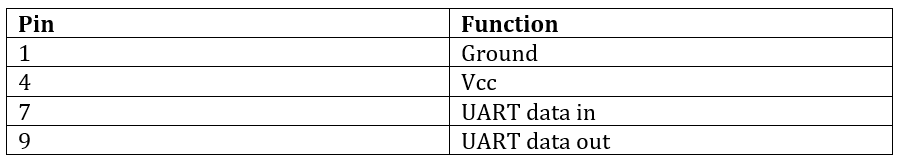
\includegraphics[width=0.75\linewidth]{./figures/tablepins}
    \caption{Table of pins used}
\end{figure}
\noindent
The transceiver has a wide range of settings that can be customised for different missions and because of this is used extensively in balloon launches. The data rate ranges from 4 Kbits/s to 250 Kbits/s and this can be set or dynamically change depending on the signal. The line of sight range that will be utilised has been recorded between 40km – 60km, making it ideal for a balloon launch which normally ascends to 30km. An air speed of 64kps will give a range of about 40km depending on antenna. If the air speed is set to be lower, the range of the wireless link increases but the amount of data that you can send will be limited. 
\begin{figure}[H]
    \centering
    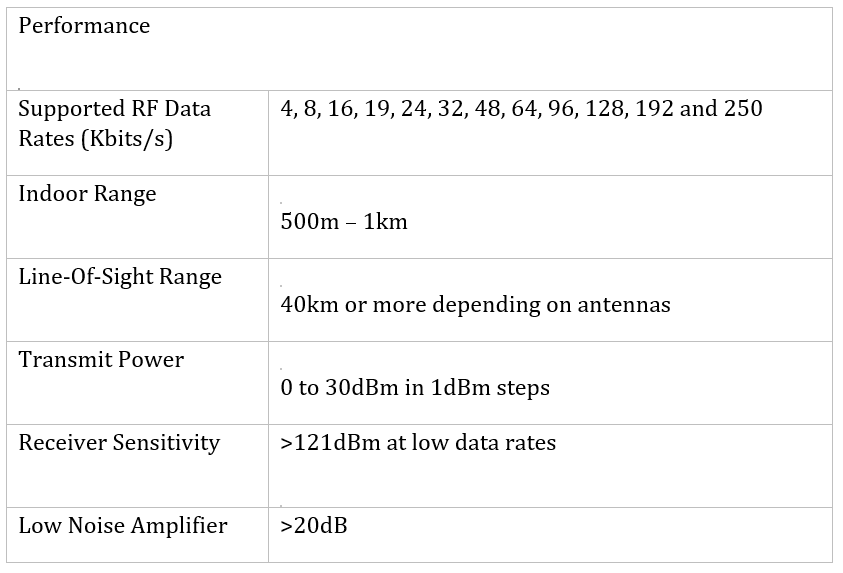
\includegraphics[width=0.9\linewidth]{./figures/performance}
\end{figure}
\noindent
The RFD900+ operates within the frequency band of 902 MHz-928MHz and uses frequency hopping spread spectrum (FHSS) to improve its immunity to interference. 
\begin{figure}[H]
    \centering
    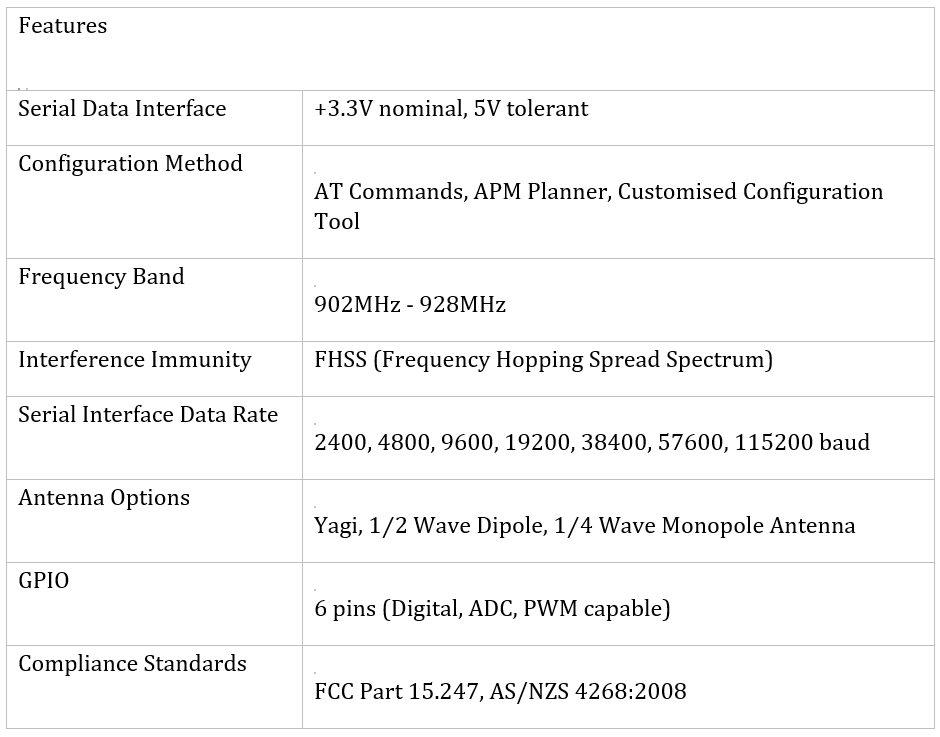
\includegraphics[width=0.9\linewidth]{./figures/features}
\end{figure}
\noindent
The configuration that was chosen includes a baud rate of 57600 with no parity, 8 data bits and 1 stop bit. This was chosen to maximise the data send back to the ground station whilst maintaining a solid link margin.
\begin{figure}[H]
    \centering
    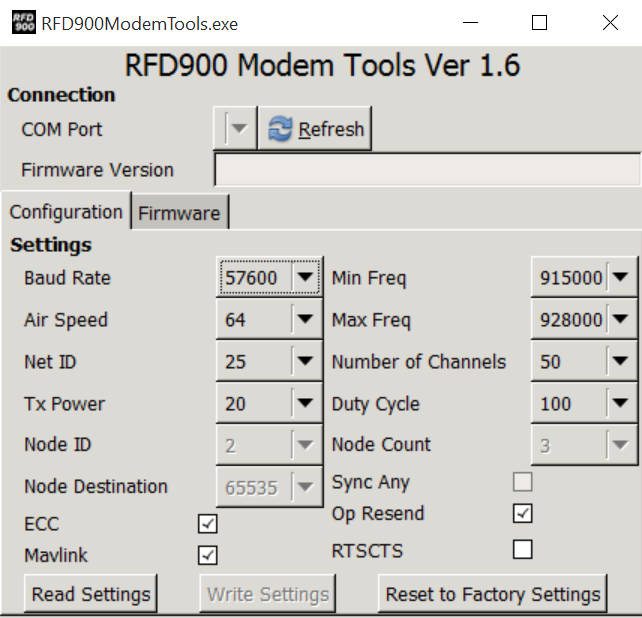
\includegraphics[width=0.75\linewidth]{./figures/rfd2}
    \caption{Settings used with transciever}
\end{figure}
\noindent
To increase the gain on both ends of the transmission, different antennas will be used at the ground station compared to the satellite. At the ground station we will utilise a yagi antenna. Yagi antennas are recommended for Ground-Station applications due to their size. They have approximately 6dBi gain and give significant link budget improvement when compared to standard dipole, or monopole antennas. 
\noindent
On the satellite we will use two quarter wave antennas. The choice was between this and half wave dipole antennas but the quart wave was declared superior due to it’s small size. Quarter Wave Monopole Antennas are recommended for air-borne, or space constrained applications. They are required to be mounted on a ground plane of approximately 20cm diameter or more to operate as intended.
\begin{figure}[H]
    \centering
    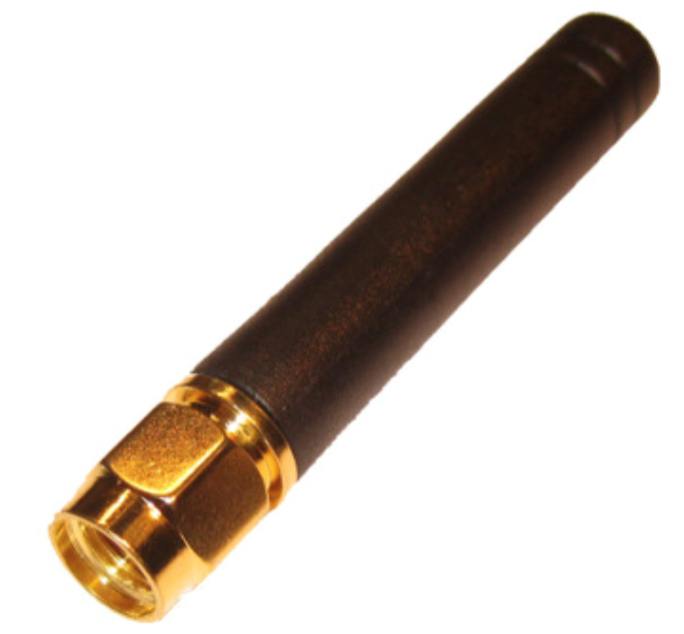
\includegraphics[width=0.6\linewidth]{./figures/antennae}
    \caption{Quarter Wave Monopole Antenna}
\end{figure}
\noindent
The RFD900 has two antenna ports and firmware which supports diversity operation of antennas. During the receive sequence the modem will check both antennas and select the antenna with the best receive signal. In the case of only one antenna connected, it will automatically select the port with the antenna connected. Testing by Silicon Labs has shown that link budgets can be improved in the order of 6-8dB by employing a diversity scheme.

\noindent 
Polarisation diversity is the case where the antennas are perpendicular to each other. i.e. one vertical, and one horizontal. This is effective in reducing multipath effects which affect one or the other polarisation. We will utilise this principle and set the antennas at a 90-degree angle to each other.

\noindent
The RFD900 can be implemented in either simple pair between two nodes or a multipoint network. In our case we have opted to use the multipoint network to allow the satellites to communicate in the air, relaying their position to aid in recovery. The following is an example of a 5 node network that will be ideally implemented. The network consists of Node 0, the ground station, Node 1, the mother satellite, and the remaining nodes are the other satellites. This structure has not been confirmed as the satellites participating in the launch is yet to be decided.
\begin{figure}[H]
    \centering
    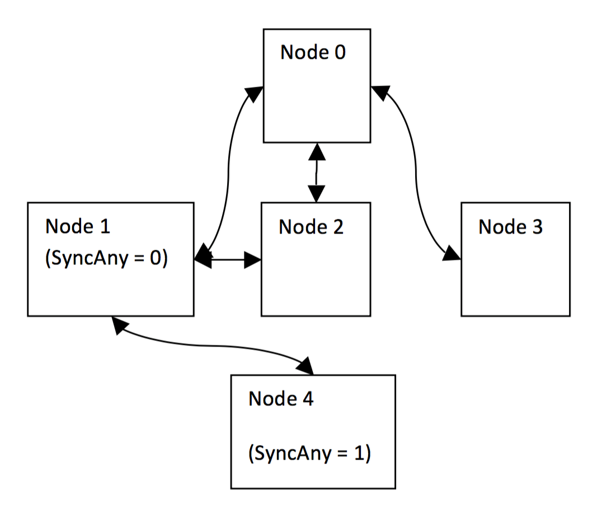
\includegraphics[width=0.7\linewidth]{./figures/nodes}
    \caption{Five-node Network Setup}
\end{figure}

\paragraph{Ground Station}
Mobile ground station utilizing the same model rfd900+ transceiver connected to a yagi antenna. Yagi antennas are recommended for Ground-Station applications due to their size. They have approximately 6dBi gain and give significant link budget improvement when compared to standard dipole, or monopole antennas. 

\noindent
The system has been set up to receive a number of commands from the ground station and act upon them. This allows it to be controlled by an operator and gives it superior functionality. The list of commands is as follows:

\noindent
User Commands
\begin{enumerate}
    \item	SET/GET TRANSMIT ON/OFF - Sets transmit to on or off
    \item	SET/GET MODE [mode]  - Sets the mode of the satellite
    \item	DOWNLOAD PAYLOAD - Download all scientific data that hasn’t been sent yet
    \item	SET PICTURE RATE - Set how often pictures are taken
    \item	SET [variable] [value] - Change the value for specific variables in code
    \item	RESET - Causes the device to reset
    \item	DELETE [date] - delete data before the given date
    
\end{enumerate}

\subsection{Link Budget Summary}
After calculating the link budget for the satellite in orbit we now have a much larger factor of safety as the free space path loss is reduced by 21 dB to 101 dB, giving us a larger margin, even considering the change in transceiver. The RFD 900+ has been used numerous times successfully for balloon launch, thereby confirming the margin is adequate. The assumptions made with the link budget include clear sky with normal humidity and a temperature of 30 degrees Celsius.
\begin{figure}[H]
    \centering
    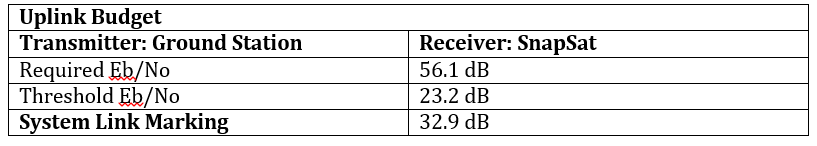
\includegraphics[width=\linewidth]{./figures/uplink}
    \caption{Uplink budget}
\end{figure}
\begin{figure}[H]
    \centering
    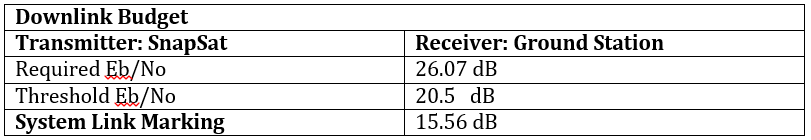
\includegraphics[width=\linewidth]{./figures/downlink}
    \caption{Downlink budget}
\end{figure}

\newpage
\section{Thermal Control Subsystem}
The method of developing thermal control used for SnapSat considers the following simplified model of the satellite. The main body is idealised as a system dissipating heat (located at the centre of the CubeSat) to the boundary located on the face of the CubeSat. This boundary is exposed to the outer environment. Energy conservation laws require that in steady state, the heat dissipated by the internal electronics is equal to that transferred tot he boundary. Thus, the heat from internal dissipation added to the heat adsorbed from the outside is equal to the heat rejected to space. The general governing equation is
\begin{equation}
    Q_{1\rightarrow2} = K_{1\rightarrow2}(T_a - T_2)
    \label{eqn:Qconduction}
\end{equation}  
\noindent
\begin{align}
    \text{Where}\quad Q &= \text{heat exchange (Watts)} \nonumber\\
    K &= \text{proportionality factor constant (Watts/Kelvin)} \nonumber\\
    T &= \text{temperature of bodies (Kelvin)} \nonumber
\end{align}
\noindent
between bodies 1 and 2. Additionally, the heat radiated from a blackbody surface of temperature $T$ is given by 
\begin{equation}
    Q_r = KT^4
    \label{eqn:Qradiation}
\end{equation} 
\noindent
Where the proportionality factor depends on physical constants, the material properties, surface conditions and geometry. A schematic of the incoming thermal radiation on the CubeSat in Low-Earth Orbit (LEO) is shown below.
\begin{figure}[H]
    \pic{0.8}{./figures/thermaloverview}{Incoming thermal radiation on the satellite}\label{fig:incomingradiation}
\end{figure}

\subsection{The Three Modes of Heat Transfer}
The first law of thermodynamics states that the internal energy change on a system is equal to the amount of heat added subtracted by the amount of work done. The work done by the satellite on its environment is zero in out case, so the change in energy becomes
\[ \cfrac{dU}{dt} = Q = A\,\rho\,c_p\,\cfrac{dT}{dt}\,dx \]
\noindent
\begin{align}
\text{Where}\quad Q &= \text{heat added (Watts)} \nonumber\\
A &= \text{cross-sectional area (m$^2$)} \nonumber\\
\rho &= \text{density of material (kg/m$^3$)} \nonumber\\
c_p &= \text{specific heat capacity (J/kg K)} \nonumber\\
T &= \text{temperature (K)} \nonumber\\
dx &= \text{incremental length (m)} \nonumber
\end{align}
Is is dependent on the physical and geometric properties of the satellite and the change in temperature. The total heat balance for the satellite is then given by the heat flux entering the system minus the flux leaving the system. These are characterised by the modes of heat transfer below.
\subsubsection{Convection}
Convection is the heat transfer between a solid surface and flowing fluid. This is of importance during mission launch, however does not apply in a space environment. Convection considerations were ignored for this design.
\subsubsection{Conduction}
Thermal energy transfer within a material due to vibrating atoms - for example if the material is heated in one location, conduction is the method by which it spreads to the rest of the material. This is most important for on-board electronics, the rate of heat transfer is given by 
\[ Q_{conduction} = \cfrac{kA}{\Delta x}\,(T_1-T_2) \]
\noindent
which is the same as equation~\ref{eqn:Qconduction}. The heat transfer depends on the area of the satellite normal to the direction of heat transfer $A$, the thermal conductivity $k$ and the temperature differential $T$.
\subsubsection{Radiation}
Perhaps the most complex form of heat transfer is radiation, where all bodies above 0K emit and absorb electromagnetic energy. We consider each body as a perfect emitter (black body) and integrate the emitted energy across all wavelengths, this gives
\begin{equation}
E_{bb} = \epsilon\sigma\,T^4
\end{equation}
measured in Watts/m$^2$. This is the same as equation~\ref{eqn:Qradiation}, where $\sigma$ is the Stefan-Boltzmann constant. In this case, the emissivity $\epsilon$ has been added to account for the fact that the surfaces are not perfect black bodies.

\subsection{Total Incoming Radiation}
The total radiation incoming onto the satellite as it orbits is defined in figure~\ref{plot:incomingradiation} below. This assumes that the satellite is in full view of the sun 65\% of the time in each orbit.
\begin{figure}[H]
    \tikzpic{0.7}{0.35}{./figures/incomingradiation.tex}{Radiation incoming onto the satellite as it orbits}
    \label{plot:incomingradiation}
\end{figure}
\noindent
Whilst this is the incoming radiation on the satellite as a whole, it is not indicative of the amount of radiation received by each side of the satellite. As the spacecraft is attitude controlled, the lower side will be facing the Earth always and only receive solar radiation for a short period of time. The amount of solar radiation (and even Earth IR radiation) received depends on the projected area that the radiation falls upon. Corrections are found using the view factor of each side of the satellite.

\subsubsection{View Factors}\label{sec:viewfactors}
The view factor of each side of the satellite allows for the calculation of the effect of the incoming radiation. The calculation takes into account the projected amount of heat flux on each side. The view factor is of importance when considering the radiation effect of Earth's infrared and albedo. The view factor indicates the area of the panel that  radiation falls upon. Naturally, the view factor fo the panel facing the Earth is 1, whilst that of the panel facing away from the Earth is 0. The other panels lie between these values, they are listed below.

\begin{figure}[H]
    \pic{0.5}{./figures/orbit.png}{Representation of Satellite Orbit}
\end{figure}



\subsection{Spacecraft Thermal Environment}
As shown in figure~\ref{fig:incomingradiation}, the spacecraft is subject to the following heating mediums: solar radiation, Earth infra-red and Earth albedo. The amount of radiation falling upon each panel is a function of the surface absorptivity and the view factor of the panel. The panel naming convention for this section is shown below.

\subsubsection{Solar Radiation}
The incoming solar radiation on the satellite is given by
\begin{equation}
    Q_{solar} = Q_{sun}\,\alpha\cos\phi
\end{equation}
\vspace{-1cm}
\begin{align}
\text{Where}\quad Q_{sun} &= \text{solar heat flux (Watts)} \nonumber\\
\alpha &= \text{panel surface absorptivity} \nonumber\\
\phi &= \text{angle between the normal of the panel to the sun (rad)} \nonumber
\end{align}
\noindent
For each of the panels, the solar radiation intensity is shown in the figure below. The skew in four of the panels is due to the 45\deg rotation of the orbit along the $z$ Earth frame.

\begin{figure}[H]
    \tikzpic{0.9}{0.25}{./figures/SolarIncomingPanels.tex}{Solar radiation falling on each panel}
\end{figure}

\subsubsection{Earth Infrared Radiation}
The incoming radiation from the Earth is in the infrared band. This radiation is due to the effective temperature of the Earth and is a constant value for each panel. For this reason, the values will not be displayed on a graph. The incoming radiation varies from panel to panel depending only on the view factors as described in section~\ref{sec:viewfactors}. The value is given by
\begin{equation}
    Q_{Earth-IR} = \sigma T_{Earth}^4 \alpha \, VF 
\end{equation}
\vspace{-1cm}
\begin{align}
\text{Where}\quad \sigma &= 1.381 \times 10^{-23}\text{ m$^2$ kg s$^{-2}$ K$^{-1}$ (Boltmann constant)} \nonumber\\
T &= \text{effective temperature of the Earth} \nonumber\\
\alpha &= \text{panel surface absorptivity} \nonumber\\
VF &= \text{panel view factor} \nonumber
\end{align}

\subsubsection{Earth Albedo}

\subsubsection{Total Incoming Radiation Per Panel}

\begin{figure}[H]
    \tikzpic{0.8}{0.25}{./figures/TotalIncomingPanels.tex}{Total radiation falling upon panel 2}
\end{figure}





\newpage
\nocite{*}
\bibliographystyle{ieeetr}
\bibliography{bib}

\newpage
\appendix

\end{document}

%% ITEM TEMPLATES

%TABLES
%\begin{table}[H]
%    \centering
%    \caption{Maximum Expected Values of Angle of Attack Excursion}
%    \vspace{0.2cm}
%    \label{tab:maxturbulencealpha}
%    {\renewcommand{\arraystretch}{1.4}%
%        \begin{tabular}{|>{\centering\arraybackslash}m{2.5cm}|>{\centering\arraybackslash}m{2.5cm}|}
%            \hline
%            Turbulence Component & Maximum ($3\sigma$ value) \\ \hline\hline
%            $u_g$ & 0.0195\deg \\ \hline
%            $w_g$ & 1.3443\deg \\ \hline
%            $q_g$ & 0.3309\deg \\ \hline
%            All & 1.3846\deg \\ \hline
%        \end{tabular} } 
%    \end{table}